\section{Relación entre $\pi_1(X)$ y $H_1(X)$}

Recordamos que el grupo fundamental de un espacio $X$ está dado por las clases de homotopía de los mapas $f:[0,1]\to X$ con $f(0)=f(1)=x_0$ para algún punto predefinido $x_0\in X$. Estos mapas también pueden ser interpretados como $1$-símplices singulares en $X$, que además van a ser ciclos ya que $\partial f = f(1)-f(0) =0$.

Va a resultar que esta asociación de curvas cerradas a $1$-símplices singulares es un homomorfismo de grupos entre $\pi_1(X,x_0)$ y $H_1(X)$. 

Si el espacio $X$ es conexo por caminos, entonces $\pi_1(X,x_0)$ es independiente del punto base $x_0$ y lo notamos simplemente $\pi_1(X)$. En ese caso el homomorfismo anterior va a resultar sobreyectivo, y su núcleo va a ser el conmutador de $\pi_1(X)$. Por lo tanto, cuando $X$ es conexo por caminos, obtenemos un isomorfismo entre $H_1(X)$ y el abelianizado del $\pi_1(X)$, que notamos $\pi_1(X)_{ab}$. 

Veamos esto en detalle:

Sean $f, g$ dos mapas de $[0,1]$ en $X$. Notamos $f\simeq g$ si existe una homotopía de extremos fjos entre $f$ y $g$. Notamos $f\sim g$ si $f$ y $g$ son homólogos como $1$-símplices en $X$, es decir, si existe un $2$-símplice $\sum n_i\sigma_i$ en $C_2(X)$ tal que $\partial\sum n_i\sigma_i = f-g$.

Primero que nada queremos definir una función $h:\pi_1(X,x_0)\to H_1(X)$ que potencialmente sea un homomorfismo de grupos. Dada una clase $[f]_{\pi_1}$ en $\pi_1(X,x_0)$, consideramos un representante de esa clase $f:[0,1]\to X$ y definimos $h([f]_{\pi_1}):=[f]_{H_1}$ como la clase de $f$ en el primer grupo de homología.

Observemos algunas características de estas relaciones.

\begin{enumerate}[wide, labelwidth=!, labelindent=0pt]
    

\item\label{ab1} Si $f$ es la función constante, entonces $f\sim 0$. Esto se debe a que el mapa constante $\sigma:\Delta^2\to X$ es un $2$-símplice singular cuyo borde coincide con $f$. 

Explícitamente, si $f(x)=x_0$ para todo $x\in [0,1]$, tenemos $\sigma:\Delta^2\to X$ tal que $\sigma(x)=x_0$ para todo $x\in\Delta^2$. En ese caso, si notamos $\Delta^2 = [v_0,v_1,v_2]$, tenemos $\partial\sigma = \sigma|_{[v_1,v_2]} - \sigma|_{[v_0,v_2]} + \sigma|_{[v_0,v_1]}$ pasando por el homeomorfismo que identifica cada par $[v_i,v_j]$ con $[0,1]$ y preserva la orientación que habíamos definido para los símplices, tenemos que $\partial\sigma = f - f + f = f$.

\item Si $f\simeq g$, entonces $f\sim g$.

Para ver esto, consideramos $F:[0,1]^2 \to X$ la homotopía a extremos fijos que manda $f$ en $g$. Si llamamos $v_0,v_1,v_2,v_3$ a los vértices de $[0,1]^2$ con $v_0:=(0,0)\; , v_1:=(0,1)\; ,v_2:=(1,1)\; ,v_3:=(1,0)$, podemos subdividir $[0,1]^2$ en dos $2$-símplices $[v_0,v_2,v_3]$ y $[v_0,v_1,v_3]$ como muestra la imagen \ref{h11}.

\begin{figure}[h!]
    	\centering
    	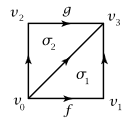
\includegraphics[width=0.25\linewidth]{img mono/abelianizado/h11.png}
    	\caption{Subdividimos el dominio de la homotopía en dos $2$-símplices}
    	\label{h11}
\end{figure}

Al restringir $f$ a cada uno de estos $2$-símplices obtenemos $2$-símplices singulares, que llamamos $\sigma_1 := F|_{[v_0,v_1,v_3]}$ y $\sigma_2 := F|_{[v_0,v_2,v_3]}$.

Estos $\sigma_1$ y $\sigma_2$ cumplen 
$$\partial (\sigma_2 - \sigma_1) = \sigma_2|_{[v_2,v_3]} - \sigma_1|_{[v_1,v_3]} -\sigma_2|_{[v_0,v_3]} + \sigma_1|_{[v_0,v_3]} + \sigma_2|_{[v_0,v_2]} - \sigma_1|_{[v_0,v_1]} $$

Como la homotopía es a extremos fijos, $\sigma_1|_{[v_1,v_3]}$ y $\sigma_2|_{[v_0,v_2]}$ son constantes, y entonces por la parte (\ref{ab1}) son homólogos a $0$.

Por definición, $\sigma_1|_{[v_0,v_3]}$ y $\sigma_2|_{[v_0,v_3]}$ son la misma función, y por lo tanto su diferencia se cancela en la suma de arriba.

Esto nos deja con $$\partial (\sigma_2 - \sigma_1) = \sigma_2|_{[v_2,v_3]} - \sigma_1|_{[v_0,v_1]} = g - f$$ que es exáctamente lo que buscábamos.

\item Si tomamos la concatenación $f\cdot g$ de los caminos $f$ y $g$, se cumple que $f\cdot g \sim f+g$.

Para probar esto consideramos un $2$-símplice $\Delta^2:=[v_0,v_1,v_2]$ y definimos $\sigma:\Delta^2\to X$ como ${(f\cdot g)}\circ p$, siendo $p$ la proyección ortogonal sobre la arista $[v_0,v_2]$ y $f\cdot g:[v_0,v_2]\to X$. En ese caso $$\partial\sigma = \sigma_{[v_1,v_2]}-\sigma_{[v_0,v_2]}+\sigma_{[v_0,v_1]}$$

Analicemos cada término. 
\begin{align*}
\sigma|_{[v_0,v_1]}&=(f\cdot g)|_{p([v_0,v_1])} = (f\cdot g)|_{[v_0, (v_2-v_0)/2]} = f \\
\sigma|_{[v_1,v_2]}&=(f\cdot g)|_{p([v_1,v_2])} = (f\cdot g)|_{[(v_2-v_0)/2,v_2]} = g \\
\sigma|_{[v_0,v_2]}&=f\cdot g
\end{align*}

Por lo tanto obtuvimos que $\partial\sigma = g - (f\cdot g) + f$ y entonces $f\cdot g \sim f+g$. La imagen \ref{h12} ilustra esto.

\begin{figure}[h!]
    	\centering
    	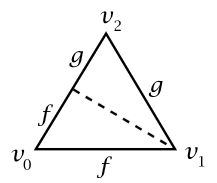
\includegraphics[width=0.25\linewidth]{img mono/abelianizado/h12.png}
    	\caption{Definimos la imagen de $\sigma$}
    	\label{h12}
\end{figure}

Recordamos que el producto en $\pi_1(X)$ de dos clases representadas por caminos $f$ y $g$ se define como la clase de homotopía de la concatenación de ambos caminos.

\end{enumerate}

